%% 
%% Copyright 2019-2020 Elsevier Ltd
%% 
%% This file is part of the 'CAS Bundle'.
%% --------------------------------------
%% 
%% It may be distributed under the conditions of the LaTeX Project Public
%% License, either version 1.2 of this license or (at your option) any
%% later version.  The latest version of this license is in
%%    http://www.latex-project.org/lppl.txt
%% and version 1.2 or later is part of all distributions of LaTeX
%% version 1999/12/01 or later.
%% 
%% The list of all files belonging to the 'CAS Bundle' is
%% given in the file `manifest.txt'.
%% 
%% Template article for cas-dc documentclass for 
%% double column output.

%\documentclass[a4paper,fleqn,longmktitle]{cas-dc}
\documentclass[a4paper,fleqn]{cas-dc}

%\usepackage[authoryear,longnamesfirst]{natbib}
%\usepackage[authoryear]{natbib}
\usepackage[numbers]{natbib}

%%%Author definitions
\def\tsc#1{\csdef{#1}{\textsc{\lowercase{#1}}\xspace}}
\tsc{WGM}
\tsc{QE}
\tsc{EP}
\tsc{PMS}
\tsc{BEC}
\tsc{DE}
%%%
% -------------------------------------------------------------------
% Pacotes para inserção de figuras e subfiguras
%\usepackage{subfig,epsfig,tikz,float}		            % Packages de figuras. 
\usepackage{graphicx}

\usepackage{caption}
\usepackage{subcaption}

\graphicspath{ {./figs/} }
% -------------------------------------------------------------------
% \usepackage{amssymb}
% -------------------------------------------------------------------
% Pacotes para inserção de tabelas
\usepackage{booktabs,multicol,multirow,tabularx,array}          % Packages para tabela
\usepackage{natbib}
\usepackage{pifont}
\usepackage{xcolor}
\usepackage{algpseudocode}
\usepackage{algorithm}
\usepackage{amsmath}
% -------------------------------------------------------------------
\PassOptionsToPackage{style=super,nolist}{glossaries}
\PassOptionsToPackage{acronym}{glossaries}
\PassOptionsToPackage{nonumberlist}{glossaries}
\usepackage{glossaries}
\newacronym{ai}{AI}{Artificial Intelligence}
\newacronym{iot}{IoT}{Internet of Things}
\newacronym{iomt}{IoMT}{Internet of Medical Things}
\newacronym{mtc}{MTC}{Machine Type Communication}
\newacronym{m2m}{M2M}{Machine To Machine}
\newacronym{tls}{TLS}{Transport Layer Security}
\newacronym{dtls}{DTLS}{Datagram Transport Layer Security}
\newacronym{iotdm}{IoTDM}{Internet of Things Device Management}
\newacronym{sdn}{SDN}{Software-Defined Networking}
\newacronym{http}{HTTP}{Hypertext Transfer Protocol}
\newacronym{coap}{CoAP}{Constrained Application Protocol}
\newacronym{mqtt}{MQTT}{Message Queuing Telemetry Transport}
\newacronym{rtt}{RTT}{Round Trip Time}
\newacronym{ap}{AP}{Access Points}
\newacronym{rsus}{RSUs}{Roadside Units}
\newacronym{qos}{QoS}{Quality of Service}
\newacronym{ccas}{CCAS}{Cluster-based Congestion-mitigating Access Scheme}
\newacronym{mtcds}{MTCDs}{Machine-type Communication Devices}
\newacronym{mtcd}{MTCD}{Machine-type Communication Device}
\newacronym{bs}{BS}{Base Station}
\newacronym{mtcg}{MTCG}{Machine-type Communication Gateway}
\newacronym{ca}{CA}{Certificate Authority}
\newacronym{p2p}{P2P}{Peer-to-Peer}
\newacronym{rest}{REST}{Representational state transfer}
\newacronym{api}{API}{Application Programming Interfaces}
\newacronym{crud}{CRUD}{Create, Retrieve, Update, Delete}
\newacronym{ae}{AE}{Application Entity}
\newacronym{aes}{AEs}{Application Entities}
\newacronym{cnt}{CNT}{Container}
\newacronym{cnts}{CNTs}{Containers}
\newacronym{cin}{CIN}{Container Instance}
\newacronym{cins}{CINs}{Container Instances}
\newacronym{sub}{SUB}{Subscription}
\newacronym{subs}{SUBs}{Subscriptions}
\newacronym{etsi}{ETSI}{European Telecommunications Standards Institute}
\newacronym{pi}{PI}{Parent Identifier}
\newacronym{cse}{CSE}{Common Services Entity}
\newacronym{ram}{RAM}{Random Access Memory}
\newacronym{json}{JSON}{JavaScript Object Notation}
\makeglossaries
% -------------------------------------------------------------------
\usepackage[utf8]{inputenc} % The default since 2018
\DeclareUnicodeCharacter{200B}{{\hskip 0pt}}
% -------------------------------------------------------------------
\begin{document}
\let\WriteBookmarks\relax
\def\floatpagepagefraction{1}
\def\textpagefraction{.001}
\shorttitle{Tiny oneM2M C Language API}
\shortauthors{Pereira Rafael et~al.}

\title [mode = title]{Tiny oneM2M C Language API}

\credit{Conceptualization of this study, Methodology, Software}

\author[1]{Rafael Pereira}[type=editor,
                        %auid=000,bioid=1,
                        linkedin=rafaelmendespereira,
                        orcid=0000-0001-8313-7253]
%\cormark[1]
%\fnmark[1]
\ead{rafael.m.pereira@ipleiria.pt}

\author[1]{Carla Mendes}[type=editor,
                        %auid=000,bioid=1,
                        linkedin=carla-mendes-5b3586233,
                        orcid=0000-0001-7138-7124]
%\cormark[1]
%\fnmark[1]
\ead{carla.c.mendes@ipleiria.pt}

\author[1]{Ana Cruz}[type=editor,
%auid=000,bioid=1,
linkedin=ana-cassia-vasconcelos-cruz10,
orcid=0009-0002-4169-7644]
%\cormark[1]
%\fnmark[1]
\ead{ana.v.cruz@ipleiria.pt}

\address[1]{Computer Science and Communications Research Centre, School of Technology and Management, Polytechnic of Leiria, 2411-901 Leiria, Portugal}

\begin{abstract}
 The \gls{iot} has revolutionized the way we interact with the environment by connecting everyday objects to the digital world, and \gls{m2m} communication is a key aspect of the \gls{iot}, enables devices to exchange data and collaborate autonomously, leading to intelligent and automated systems. 
 In this paper, we present TinyOneM2M: an implementation of the OneM2M standard using a low-level programming language-based approach, to address the limitations associated with high-level language implementations. Our implementation aims to enhance performance and reduce memory overhead. Through different tests, we evaluate the usability, scalability, and reliability of the solution in various scenarios. 
 The results demonstrate that our TinyOneM2M solution offers seamless interoperability and scalability to \gls{iot} and general applications on several Linux-based operating systems, even in resource-constrained scenarios.

\end{abstract}

%\begin{graphicalabstract}
%
\includegraphics{figs/grabs.pdf}
%\end{graphicalabstract}
%
%\begin{highlights}
%\item Research highlights item 1
%\item Research highlights item 2
%\item Research highlights item 3
%\end{highlights}

\begin{keywords}
Internet of Things \sep OneM2M \sep Scalability \sep 
\end{keywords}


\maketitle

\section{Introdution}

The \gls{iot} encompasses a vast network of diverse entities, including tags, sensors, embedded devices, handheld devices, and backend servers. It enables the development of novel services and applications across various domains such as civil transportation, electric power grids, medical treatment, and industrial and home automation \cite{kim_m2m_2014}. 

\gls{m2m} denotes technologies that enable communication and networking of different devices and is a part of the field of \gls{iot}. While the \gls{iot} focuses on the interconnection of physical objects and their interaction with humans, the \gls{m2m} system focus towards seamless connectivity. It involves automated systems where devices autonomously gather data (e.g., temperature, humidity, speed, position, heartbeat) from remote sources, exchange information, and execute actions based on control messages. These operations generally occur without or with minimal human intervention, utilizing public network infrastructures. Consequently, the \gls{m2m} system plays a crucial role in realizing the full potential of the \gls{iot} \cite{kim_m2m_2014}, \cite{lawton_machine_2004}, \cite{pticek_architecture_2015}.

\gls{m2m} systems are typically characterized by their heterogeneity, lack of structure, and loose integration, achieved through standardized communication technologies. These technologies include WiFi, Zigbee, Ethernet, and power line communications, among others. By leveraging standardized technologies, \gls{m2m} systems enable seamless interoperability among devices and simplify mass-produced, standards-compliant equipment. This approach contributes to cost-effective implementations, reducing expenses associated with system development and deployment \cite{lawton_machine_2004}, \cite{cao_survey_2016}.

The rapid expansion of \gls{m2m} technologies has compelled various standardization bodies, such as the \gls{etsi}, to establish \gls{m2m} standards, resulting in the emergence of multiple standards (e.g \gls{etsi} \gls{m2m} and OneM2M). Consequently, the OneM2M initiative was established to develop a unified global specification and standard for \gls{m2m} communication \cite{pticek_architecture_2015}.

In 2008, \gls{etsi} initiated the standardization process for \gls{m2m} by examining requirements and identifying gaps in existing standards. \gls{etsi} began defining an \gls{m2m} platform that could cater to various sectors such as smart metering, e-health, transportation, manufacturing, facility management, and more. In February 2015, OneM2M introduced its first global standard. OneM2M shared the same objective as \gls{etsi} \gls{m2m} but aimed to achieve it on a global level \cite{pticek_architecture_2015}. 

Therefore, the oneM2M \footnote{OneM2M official page: \url{https://www.onem2m.org/}} standard aims to establish uniformity in the communication between devices, servers, and applications by offering a standardized \gls{m2m} service. It defines a platform centered around the concept of resources and \gls{rest} \gls{api}. Moreover, it encompasses over a dozen Common Service Functions such as registration, subscription, discovery, and data management, among others \cite{onem2m_standard}.

In this paper, we present a novel implementation of the OneM2M standard using a low-level programming language to address the limitations of high-level language-based implementations. Our approach is purposefully designed to be lightweight, catering to weak computational systems with limited processing power and memory capacity, reducing memory overhead and increasing control over hardware resources. By focusing on key challenges associated with \gls{mtc} gateways, such as protocol interoperability, scalability, and latency, our implementation aims to provide a robust and efficient solution for the evolving \gls{iot} landscape.

The remainder of this paper is organized as follows: Section \ref{relatedWork} provides a comprehensive review of the related work in current \gls{m2m} implementations, discussing various programming languages. In section \ref{architecture}, we delve into the system architecture of our TinyOneM2M software, discussing the specific modules that constitute it where we present three scenarios: Home Gateway, Single Device (peer-to-peer), and Cloud, highlighting how the architecture adapts to each scenario. In section \ref{sec:tinyonem2msolution}, we provide a comprehensive overview of our implementation of the OneM2M standard version 5.1, detailing the system resources that form the foundation of our solution. The testing mechanisms employed to examine the TinyOneM2M solution under various scenarios are detailed in section \ref{tests}. Section \ref{sec:lessonsLearned} encompasses the acquired knowledge and reflective insights gained throughout the system's development. Finally, in section \ref{conclusion}, we conclude the paper by summarizing the key findings and contributions, and we highlight potential future research directions.

\section{Related work}
\label{relatedWork}

OneM2M provides a standardized framework and protocols to enable interoperability between diverse \gls{iot} devices. It can be regarded as an overarching framework that facilitates the implementation of \gls{m2m} solutions, allowing for seamless communication and integration of various machine-to-machine interactions within an \gls{iot} ecosystem \cite{onem2m_standard}. Therefore, in this section, we will provide an overview of the current state-of-the-art in \gls{m2m} implementations, highlighting the advantages and disadvantages of various programming languages and architectural choices.

Rubi et al. \cite{Rubi2019} propose an \gls{iomt} platform with a cloud-based electronic health system that collects data from various sources and relays it through gateways or fog servers. The platform enables data management, visualization of electronic records, and knowledge extraction through big data processing, machine learning, and online analytics processing. Additionally, it offers data sharing services for third-party applications, improving healthcare services and interoperability.

The authors in \cite{Volkov2017} conducted \gls{iotdm} service testing for smart city management, focusing on the ecological situation in Saint-Petersburg's central district, using an \gls{sdn} network infrastructure. They developed a hierarchical model and \gls{iot} traffic generator in compliance with oneM2M specifications and implemented \gls{http}, \gls{coap}, and \gls{mqtt} protocols. Their findings suggested that \gls{http} is the most suitable protocol for registering \gls{iot} devices to the \gls{iotdm} service, while \gls{mqtt} is optimal for transmitting sensor data. The authors concluded that the \gls{sdn} approach significantly reduces the \gls{rtt} parameter, demonstrating its potential in managing \gls{iot} traffic in smart city environments.

Soumya et al. \cite{Datta2015} explore Fog Computing as a consumer-centric \gls{iot} service deployment platform, particularly for connected vehicles and intelligent transportation systems requiring low latency, high mobility, real-time data analytics, and wide geographic coverage. They present an \gls{iot} architecture for connected vehicles, integrating Fog Computing platforms into oneM2M standard architecture. The architecture comprises virtual sensing zones, \gls{ap}, \gls{rsus}, \gls{m2m} gateways, and cloud systems. Fog Computing enables consumer-centric services such as \gls{m2m} data analytics with semantics, discovery of \gls{iot} services, and management of connected vehicles. The paper highlights the advantages of Fog Computing, including reduced latency, improved \gls{qos}, real-time data analysis, and actuation for superior user experience and consumer-centric \gls{iot} products.

This paper \cite{Liang2018} presents a \gls{ccas} that addresses the issue of collision and access efficiency in \gls{m2m} communications. The authors propose a modified spectral clustering algorithm to form clusters based on the location and service requirements of \gls{mtcds}, ensuring that devices with similar requirements are grouped together. They also develop an \gls{mtcg} selection algorithm that considers the delay requirements of \gls{mtcds} and selects an \gls{mtcg} with the appropriate forwarding threshold. The proposed CCAS divides the data transmission process into an \gls{mtcd}-\gls{mtcg} stage and an \gls{mtcg}-\gls{bs} stage to reduce collision probability and increase the number of successfully received packets, without causing additional average access delays for \gls{mtcds}. The paper includes a theoretical analysis of the \gls{mtcg} aggregation and forwarding process, as well as performance evaluations through simulations.

The paper \cite{Thielemans2019} proposes a resource-efficient secure implementation of OneM2M based on C programming language for \gls{iot}, while also performing an analysis of the OneM2M architecture and protocols. Furthermore, the authors highlight the relevance of a lightweight implementation using optimized data structures and algorithms for \gls{iot} devices with limited resources and propose a solution that can reduce computational costs and processing time. Secure communication protocols such as \gls{tls} and \gls{dtls}, as well as authentication and encryption mechanisms, were used to ensure security. The authors also suggested that the cryptography algorithms chosen must be lightweight to reduce the computational burden on \gls{iot} devices. The evaluation of this implementation meant using a set of benchmarks while comparing the developed OneM2M implementation with existing ones. Results showed that, in terms of memory usage and processing time, the author's proposed implementation of OneM2M using C language is more resource-efficient.

The authors in \cite{Benoygopal2021} present a secure authentication and access control scheme for OneM2M-based \gls{iot} systems. Moreover, propose an approach to address the challenge of identity and access management in large-scale \gls{iot} systems. The proposed scheme is based on the role-based access control model, where system administrators can define access policies based on the roles of the users. Their scheme entails a secure authentication and authorization mechanism based on certificates, which are issued by a trusted \gls{ca}. The evaluation process used a prototype implementation of the OneM2M standard and compared it with existing access control schemes. Therefore concluding that their scheme achieves better performance and scalability while providing a flexible and fine-grained access control mechanism. However, the proposed scheme contains security and privacy issues for which the authors presented several countermeasures to mitigate them.

The paper \cite{Kim2018} discusses the design, implementation and evaluation of an interoperable platform for the Internet of Things \gls{iot} using the OneM2M standard, where the authors focused on implementing the standard using C language. Moreover, the authors discussed how their C implementation handles registration, discovery and subscription-resource management tasks while proposing optimizations to improve performance. Experiments were designed to assess the scalability, reliability, and processing time with different loads and data sizes. Those experiments concluded that the C implementation of OneM2M achieved better performance than other implementations regarding response time and memory usage. Regarding security, the paper also details oneM2M's security features, namely, authentication, authorization, and confidentiality, how the C implementation handles these features and how to improve the platform's security. Interoperability features, such as standardized interfaces and protocols, and their C implementation were also detailed in the paper since one of oneM2M's main objects must be the interoperability between different \gls{iot} platforms and devices.

% https://www.scopus.com/results/results.uri?sort=plf-f&src=s&st1=%28onem2m+OR+mtc%29+and+%22API%22&sid=2e6f61fce202fa9e6635e553544fee3c&sot=b&sdt=b&sl=40&s=TITLE-ABS-KEY%28%28onem2m+OR+mtc%29+and+%22API%22%29&origin=searchbasic&editSaveS=&yearFrom=Before+1960&yearTo=Present

\section{Architecture}
\label{architecture}

The architecture of TinyOneM2M, a compact, cross-platform, and easy-to-use implementation of the OneM2M standard \cite{onem2m_standard}, is meticulously designed to adapt to various scenarios. The flexible architecture supports different modes of operation, allowing it to integrate seamlessly into existing infrastructure. This section details the system architecture and the specific modules that constitute the TinyOneM2M software.

\subsection{System Architecture}

The system architecture of TinyOneM2M is developed considering the diverse range of scenarios that could arise in \gls{iot} settings. Three primary scenarios have been identified where TinyOneM2M can be effectively employed, namely, the Home Gateway Scenario, the Single Devices Scenario (\gls{p2p}), and the Cloud Scenario.

\begin{figure}[htb]
     \centering
     \begin{subfigure}[h]{7cm}
         \centering
         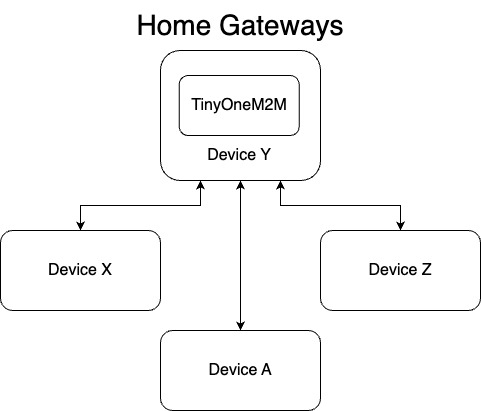
\includegraphics[width=6cm]{HomeGatewaysScenario.jpg}
         \caption{Home Gateway Scenario.}
         \label{fig:hgw}
     \end{subfigure}
     \hfill
     \begin{subfigure}[h]{7cm}
         \centering
         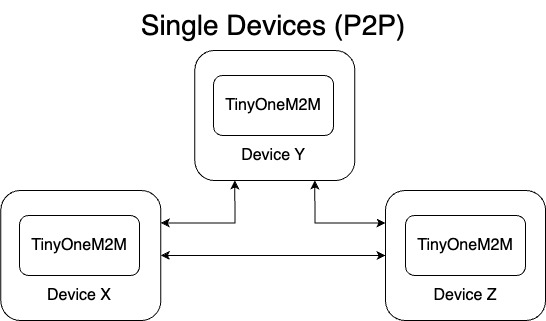
\includegraphics[width=6cm]{SingleDevicesScenario.jpg}
         \caption{Single Devices Scenario (\gls{p2p}).}
         \label{fig:sdc}
     \end{subfigure}
     \hfill
     \begin{subfigure}[h]{7cm}
         \centering
         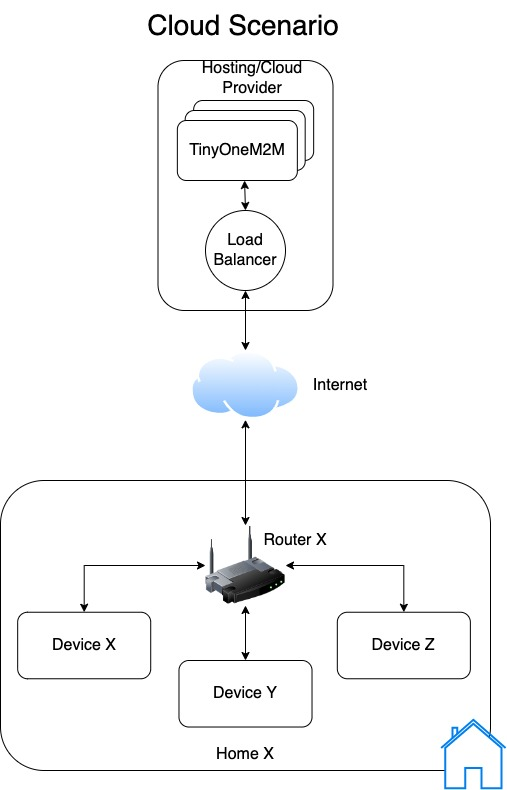
\includegraphics[width=6cm]{CloudScenario.jpg}
         \caption{Cloud Scenario.}
         \label{fig:cs}
     \end{subfigure}
     \caption{TinyOneM2M System Architecture.}
     \label{fig:scenarios}
\end{figure}

In the Home Gateway Scenario (Figure \ref{fig:hgw}), TinyOneM2M serves as a central gateway within a home network, facilitating communication between different devices in the network. This centralized approach allows for efficient data transfer and coordination between devices.

The Single Devices Scenario (Figure \ref{fig:sdc}) represents a decentralized, \gls{p2p} approach where each device contains its instance of TinyOneM2M. This approach allows devices to communicate directly with each other, enhancing scalability and data transfer efficiency by eliminating the need for a central point of communication.

In the Cloud Scenario (Figure \ref{fig:cs}), TinyOneM2M is hosted on a cloud provider and can be distributed in several machines/instances and be managed by a load balancer, allowing devices to connect and communicate via the internet. This scenario facilitates large-scale, distributed \gls{iot} applications, providing the advantages of cloud computing such as high availability, scalability, and efficient data management.

\subsection{TinyOneM2M Architecture}\label{tinyonem2marchitecture}

TinyOneM2M is architected in a way that distinctly separates responsibilities across various modules, providing a robust and efficient system. Its architecture is underpinned by a seamless flow of operations that handles and processes incoming \gls{http} \gls{rest} requests, ultimately leading to action being taken, such as data persistence or triggering notifications. An overview of the architecture is depicted in Figure \ref{fig:TinyOneM2Mchitecture} and will be described in the following sections dividing each module by section.

\begin{figure*}[htbp]
	\centering
	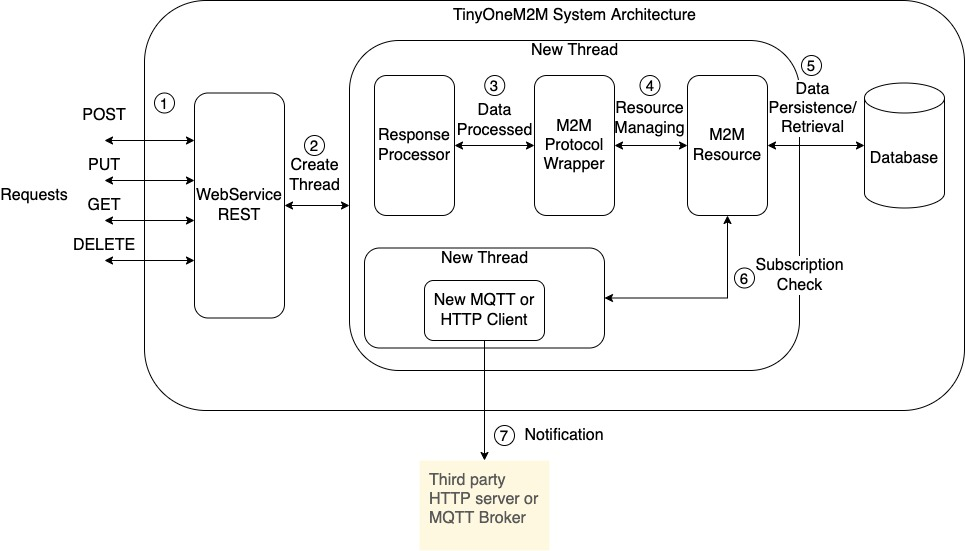
\includegraphics[width=\linewidth]{SolutionArchitecture.jpg}
	\caption{TinyOneM2M System Architecture.}
	\label{fig:TinyOneM2Mchitecture}
\end{figure*}

\subsubsection{Overview of Resource Oriented Architecture}

A crucial aspect of TinyOneM2M's system architecture, as depicted in Figure \ref{fig:systemarchitecture}, is the interaction between third-party applications and TinyOneM2M, and between TinyOneM2M and external \gls{mqtt} brokers or \gls{http} web servers. This figure outlines these interactions and the hierarchy of resources (described in Section \ref{sec:M2MResource}) within the TinyOneM2M system.

\begin{figure}[h]
	\centering
	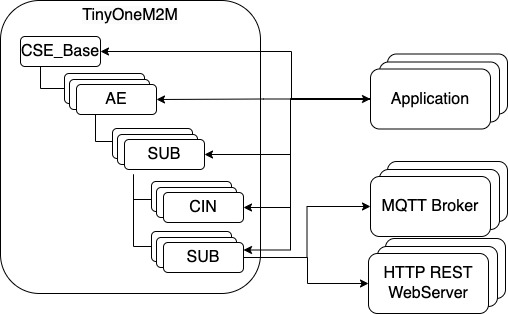
\includegraphics[width=\linewidth]{SystemArchitectuRE.jpg}
	\caption{System Architecture.}
	\label{fig:systemarchitecture}
\end{figure}

Third-party applications communicate with TinyOneM2M to create or retrieve resources. They send \gls{http} \gls{rest} requests to the \gls{rest} Webservice module in TinyOneM2M, which acts as an intermediary, accepting and processing various types of requests, including POST, GET, PUT, and DELETE. Depending on the type of request, the application can create a new resource, retrieve details of an existing resource, update a resource, or remove a resource.

TinyOneM2M also communicates with \gls{mqtt} brokers or \gls{http} WebServers, primarily for notifying about events based on subscriptions inserted into the TinyOneM2M system. If a resource is marked as notifiable changes - for instance, if a new data point is added to a monitored sensor - TinyOneM2M's Notification module creates an \gls{mqtt} or \gls{http} client to send a notification to the relevant \gls{mqtt} broker or \gls{http} server at the moment the changes happen. This notification mechanism allows applications to react promptly to changes in monitored resources, making it an integral part of many \gls{iot} scenarios, from anomaly detection in industrial settings to updates in smart home environments.

\subsubsection{WebService REST}\label{sec:archwebservice}

The \gls{rest} Webservice module in TinyOneM2M functions as the system's primary interface, accepting and processing various types of \gls{http} \gls{rest} requests. When a request is received, this module generates a new thread to manage the request, which is then passed onto the next layer for further processing.

The types of \gls{http} request that are supported by TinyOneM2M are primarily structured around \gls{crud} operations for various resources. These operations pertain to different resources identified by OneM2M standards, including \gls{ae}, \gls{cnt}, \gls{cin}, \gls{sub} resources.

For \gls{aes}, users can perform different actions on \glspl{ae} using specific HTTP requests. They can create a new \gls{ae} by sending a POST request, retrieve the details of an \gls{ae} using a GET request, update an \gls{ae} using a PUT request, and remove an \gls{ae} by issuing a DELETE request. These requests are sent to a specific URL structure, targeting the CSE\_Base and the \texttt{AE\_ResourceName}.

For \gls{cins}, the operations mirror those for \gls{aes} but are extended with an additional URL parameter to specify the \gls{cin}. These operations thus allow users to create, retrieve, and delete \gls{cins} within a specific \gls{ae} and \gls{cnt} resource.

Similarly, \gls{sub} resources can be managed with POST, GET, PUT, and DELETE requests. These requests target a specific \texttt{SUB\_ResourceName} within a specified CSE\_Base, \texttt{AE\_ResourceName}, and \texttt{CNT\_ResourceName}.

The system also provides functionality to retrieve the root resource information with a specific GET request and perform discovery operations. The discovery operation uses a GET request with query parameters to filter resources based on their type and labels. These operations can be used to retrieve general or specific information about the resources available in the system.

\subsubsection{Response Processor} \label{sec:archresponseprocessor}

The instantiated thread uses the Response Processor module to validate the request, determine the HTTP method, and conduct preliminary validations. The processed request is then forwarded to the next module for further action.

\subsubsection{M2M Protocol Wrapper}

The \gls{m2m} Protocol Wrapper is responsible for processing and validating the incoming request according to the OneM2M standard. It acts as a bridge between the protocol-specific details of the request and the \gls{m2m} resource module, ensuring that all processed requests comply with the OneM2M standard.

\subsubsection{M2M Resources}\label{sec:M2MResource}

The \gls{m2m} Resources module in TinyOneM2M is a crucial component that handles data persistence and retrieval operations. Acting as an intermediary between the incoming requests and the database, this module either persists data to the database or retrieves data from it, based on the action specified in the processed request. Additionally, it checks if the parent resource associated with the incoming request is notifiable. If it is, the module triggers a new thread for the Notification module, thus effectively bridging the communication between the client and the notification mechanisms.

This module supports different types of resources, following a hierarchical structure as prescribed by the OneM2M standard and as shown in Figure \ref{fig:hierarchy}. The CSE\_Base \gls{cse} resource sits at the root of this hierarchy, providing an entry point for all other resources in the system.

The \gls{ae} is an application-level entity that provides services to end-users. It can encapsulate \gls{cnt} and \gls{sub} resources, which provide data organization and condition-based notification services, respectively.

The \gls{cnt} resource represents a container for organizing data within \gls{ae} and other \gls{cnt} resources. It can contain other \gls{cnt}, \gls{cin}, and \gls{sub} resources, allowing an organized and hierarchical data structure.

The \gls{cin} resource, residing under a \gls{cnt}, encapsulates the actual data or content in the system. The \gls{sub} resource, which can be nested under CSE\_Base, \gls{ae}, and \gls{cnt} resources, is responsible for managing subscriptions. This enables applications to receive notifications about changes in resources they're interested in.

\begin{figure}[htbp]
	\centering
	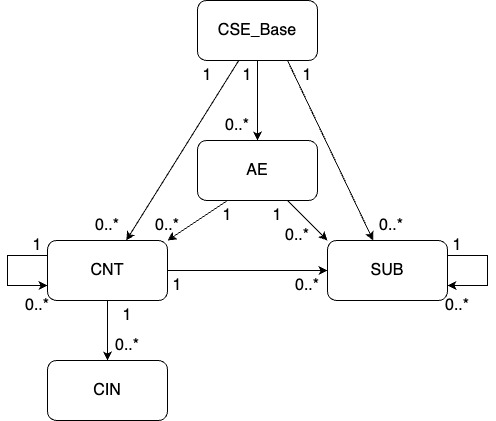
\includegraphics[width=7cm]{Hierarchy}
	\caption{TinyOneM2M supported resources hierarchy.}
	\label{fig:hierarchy}
\end{figure}

\subsubsection{Embedded Single File Database}

The TinyOneM2M system relies on an embedded single-file database for optimized data storage and retrieval. This format offers high efficiency due to its low overhead and quick access time. The system employs a denormalized structure in certain areas, an approach commonly used in database design to improve performance, even at the expense of data redundancy.

In this setup, there is one main table named \texttt{mtc}. This table in \ref{tab:database} is a combination of multiple entity types in the TinyOneM2M hierarchy, such as \gls{ae}, \gls{cin} and \gls{sub}. The attributes of these entities are represented as columns in the \texttt{mtc} table using their abbreviations, .

Looking deeper into the table structure, the \texttt{ri} (resource identifier) column serves as the primary key, providing unique identification for each record. It establishes relations with the \gls{pi} column, which refers to the \texttt{ri} of the parent record. This sets up a hierarchical relationship between records, which mirrors the resource hierarchy in the TinyOneM2M system.

The table also includes specific columns for different resource attributes. For example, \texttt{ty}, \texttt{rn}, and \texttt{et}. It also stores specific attributes for \gls{ae} like \texttt{aei}, for \gls{sub} like \texttt{nu} and \texttt{enc}, and for \gls{cin} like \texttt{con} and \texttt{cnf}.

Some columns like \texttt{cbs} (current byte size) and \texttt{mni} (maximum byte size) are used for handling quotas and limits in the TinyOneM2M system. For instance, \texttt{cbs} and \texttt{mbs} are related to the storage size occupied by \gls{cin} resource inside a \gls{cnt} and its maximum allowed size, respectively.

The \texttt{mtc} table also includes columns like \texttt{url}, \texttt{lbl}, \texttt{acpi}, \texttt{daci}, and \texttt{poa} (point of access), which store various types of information required for OneM2M standard operations.

To optimize read operations and streamline data retrieval, we have introduced a blob column that stores the \gls{json} object associated with each resource. This approach eliminates the need to select all the columns from the table and map them to the \gls{json} object, as we can now retrieve the complete \gls{json} object directly from the blob column. By doing so, we significantly improve performance and simplify the data retrieval process. Additionally, the database employs indexes on selected columns which allows faster data retrieval and processing, a key requirement for real-time operations in \gls{iot} environments. For instance, the \texttt{sqlite\_autoindex\_mtc\_1} index on the \texttt{ri} column helps in quickly locating records based on their unique identifiers.

\begin{table}[h]
	\scriptsize
	\caption{Atributes designations.}
	\label{tab:attributesDesignations}
	\begin{tabular}{ >{\bfseries}p{1.5cm} c }
		\hline
		\textbf{Attribute Abbreviation} & \textbf{Attribute Designation} \\
		\hline \hline
		\texttt{ty} & Resource type \\
		\hline
		\texttt{ri} & Resource identifier \\
		\hline
		\texttt{rn} & Resource name \\
		\hline
		\texttt{pi} & Parent identifier \\
		\hline
		\texttt{aei} & \gls{ae} identifier \\
		\hline
		\texttt{csi} & \gls{cse} identifier \\
		\hline
		\texttt{cst} & \gls{cse} type \\
		\hline
		\texttt{api} & App identifier \\
		\hline
		\texttt{rr} & Request reachability \\
		\hline
		\texttt{et} & Expiration time \\
		\hline
		\texttt{ct} & Creation time \\
		\hline
		\texttt{lt} & Last modified time \\
		\hline
		\texttt{url} & Url \\
		\hline
		\texttt{lbl} & Labels \\
		\hline
		\texttt{acpi} & Access control policy IDs \\
		\hline
		\texttt{daci} & Dynamic authorization consultation IDs \\
		\hline
		\texttt{poa} & Point of access \\
		\hline
		\texttt{srt} & Serialization time \\
		\hline
		\texttt{blob} & Blob \\
		\hline
		\texttt{cbs} & Current byte size \\
		\hline
		\texttt{cni} & Current number of instances \\
		\hline
		\texttt{mbs} & Maximum byte size \\
		\hline
		\texttt{mni} & Current number of instances \\
		\hline
		\texttt{st} & State tag \\
		\hline
		\texttt{cnf} & Content info \\
		\hline
		\texttt{cs} & Content size \\
		\hline
		\texttt{con} & Content \\
		\hline
		\texttt{nu} & Notification URI \\
		\hline
		\texttt{enc} & Event notification criteria \\
		\hline
	\end{tabular}
\end{table}

\begin{table}[h]
\scriptsize
\caption{Database structure.}
\label{tab:database}
\begin{tabular}{ >{\bfseries}p{1.5cm}cp{3cm} }
    \hline
    \textbf{Column Name} & \textbf{Type} & \textbf{Reference} \\
    \hline \hline
    \texttt{ty} & INTEGER & - \\
    \hline
    \texttt{ri} & TEXT & PRIMARY KEY \\
    \hline
    \texttt{rn} & TEXT & - \\
    \hline
    \texttt{pi} & TEXT & REFERENCES mtc(ri) ON DELETE CASCADE \\
    \hline
    \texttt{aei} & TEXT & - \\
    \hline
    \texttt{csi} & TEXT & - \\
    \hline
    \texttt{cst} & INTEGER & - \\
    \hline
    \texttt{api} & TEXT & - \\
    \hline
    \texttt{rr} & TEXT & - \\
    \hline
    \texttt{et} & DATETIME & - \\
    \hline
    \texttt{ct} & DATETIME & - \\
    \hline
    \texttt{lt} & DATETIME & - \\
    \hline
    \texttt{url} & TEXT & - \\
    \hline
    \texttt{lbl} & TEXT & - \\
    \hline
    \texttt{acpi} & TEXT & - \\
    \hline
    \texttt{daci} & TEXT & - \\
    \hline
    \texttt{poa} & TEXT & - \\
    \hline
    \texttt{srt} & TEXT & - \\
    \hline
    \texttt{blob} & TEXT & - \\
    \hline
    \texttt{cbs} & INTEGER & - \\
    \hline
    \texttt{cni} & INTEGER & - \\
    \hline
    \texttt{mbs} & INTEGER & - \\
    \hline
    \texttt{mni} & INTEGER & - \\
    \hline
    \texttt{st} & INTEGER & - \\
    \hline
    \texttt{cnf} & TEXT & - \\
    \hline
    \texttt{cs} & INTEGER & - \\
    \hline
    \texttt{con} & TEXT & - \\
    \hline
    \texttt{nu} & TEXT & - \\
    \hline
    \texttt{enc} & TEXT & - \\
    \hline
\end{tabular}
\end{table}

\subsubsection{Notifications}

The Notification module is responsible for sending notifications based on subscription resources. When a resource (e.g. Container) contains a subscription directly inside and other resource (e.g. Content Instance) is created directly inside the resource (e.g. Container) an \gls{mqtt} or \gls{http} client is asynchronous created to send a notification to the respective third-party \gls{mqtt} or \gls{http} broker.

\section{Implementation of TinyOneM2M Solution} \label{sec:tinyonem2msolution}

Our solution adheres to the OneM2M standard version 5.1 \footnote{\url{https://www.onem2m.org/technical/published-specifications\#listofreleases}}, implementing a set of key resources integral to our intended functionalities. We opted for the implementation of the resources CSE\_Base, \gls{ae}, \gls{cnt}, \gls{cin}, and \gls{sub}. The implementation of TinyOneM2M is designed with a strong focus on the system architecture presented in Figure \ref{fig:TinyOneM2Mchitecture} in section \ref{architecture}. Each component of the architecture has a corresponding implementation detail which we aim to elucidate throughout this section.

The development of the TinyOneM2M solution was carried out using the C language. There are several reasons for this choice. Firstly, C is highly portable and efficient, making it ideal for \gls{iot} applications where devices can have varied processing capabilities. It also offers low-level access to memory, which allows fine-tuned control over system resources. However, C also has some disadvantages. It lacks the built-in object-oriented features found in languages like C++ or Python, which can lead to more complex code structures for large systems. Moreover, the C language places the burden of memory management on the developer, which, if not executed with caution, can give rise to potential issues and challenges.

To gauge our level of compliance with the OneM2M standard, we quantified the degree of our implementation based on each resource. We calculated the percentage of implementation by comparing the number of implemented attributes to the total number of attributes suggested by the standard, all multiplied by one hundred.

Based on this calculation, we estimate that our solution covers approximately 57\% of the standard on average. A detailed breakdown of this calculation, per resource, will be further elucidated in the section \ref{sec:m2mresources}.

Our implementation is designed to ensure compatibility with services utilizing the OpenMTC \footnote{\url{https://github.com/OpenMTC/OpenMTC}} SDK, an open-source framework that provides an OneM2M-based version 1.1 platform. This interoperability is possible because the \gls{rest} requests in our implementation have the same structure as those in the OpenMTC implementation and return similar error codes.

Throughout the development process, we've leveraged a variety of external and non-native libraries. The specific libraries used, along with their corresponding versions, will be duly referenced in the following sections. We believe this level of transparency is crucial to understand the depth and scope of our work.

In the subsequent sections, we will delve into greater detail about our implementation, covering different aspects of our TinyOneM2M solution, and providing a comprehensive view of what was achieved.

\subsection{WebService REST}

The WebService REST module, as discussed in Section \ref{sec:archwebservice}, plays a vital role in our TinyOneM2M solution. It functions as the primary communication hub, receiving \gls{http} requests and handling client connections. This module is pivotal to our architecture, acting as the gateway through which third-party systems and applications interact with our TinyOneM2M solution.

The implementation of this module is carried out with the pthread library for thread creation, and the native socket library for setting up and managing the \gls{rest} Webserver. When the webserver detects new clients, it accepts them and launches a new thread. This thread is responsible for reading the content of the request and executing the complete request processing workflow.

To manage webserver routes, a double-sorted list was employed. This list uses the alphabetical order of the resource path as the key for sorting and simple fields to facilitate resource queries. The resource path, which is a composite of the \texttt{resource name} of the resources in the resource hierarchy, is immutable.

Upon the application's start, the database is scanned to construct the ordered double list, which is subsequently stored in \gls{ram}. This strategy ensures enhanced query efficiency whenever the existence of a request's resource path needs to be verified. When a resource is inserted or deleted, the list is updated accordingly.

However, the use of pthread and the native socket library present a few limitations. While efficient, these libraries may not offer optimal compatibility for systems like Windows, thus limiting the platform independence of our solution. A potential enhancement could be the use of a cross-platform library, such as Drogon \footnote{\url{https://github.com/drogonframework/drogon}} for C++, which could offer non-blocking operations for the \gls{http} server.

It's important to note that the algorithm for managing the double-sorted list was custom implemented by the authors. While this allowed for a tailored solution to our specific needs, a well-tested library could have been utilized for this purpose, potentially offering more robustness and efficiency. Nonetheless, our current implementation is situated within the main process and has shown competent performance in managing routes for the webserver.

\subsection{Response Processor}

As introduced in Section \ref{sec:archresponseprocessor}, the Response Processor module is central to handling the incoming content from the solution's clients. It undertakes critical tasks such as reading the content of the clients' connections, validating the routes based on the sorted double list, and processing the \gls{http} request types.

The module employs a built-in hash table to efficiently map the resources affected by the requests. The hash table provides swift access to key values, making it highly suitable for this task. It inspects and interprets the resource types encapsulated in the \gls{http} requests, facilitating the subsequent processing steps.

One important aspect to note is the static nature of the hash table. Stored in memory, the hash table remains constant for the entire lifetime of the service. This means it is built only once during the service initialization and does not change over time.

However, similar to the WebService \gls{rest} module, the algorithm to manage the hash table was also a custom implementation. Although it is designed to meet the specific needs of this application, a pre-existing, well-tested library could offer enhanced reliability and potentially better performance.

\subsection{M2M Protocol Wrapper}

As established in section \ref{architecture}, the \texttt{M2M Protocol Wrapper} is instrumental for the operation of the entire system. Its functions range from initial protocol initialization, resource discovery, and building values, to defining default values and facilitating the insertion of resources into the database.

Upon protocol initialization, the database is created and the resource CSE\_Base is populated if this has not been done previously. The resource discovery feature is 28\% implemented according to the standard, implementing 9 of the suggested 32 filters.

Table \ref{tab:discovery_attributes} describes each implemented discovery attribute:

\begin{table}[ht]
\scriptsize
\centering
\caption{Description of implemented discovery attributes}
\label{tab:discovery_attributes}
\begin{tabular}{c c p{4cm}}
\hline
\textbf{Filter Name} & \textbf{Cardinality} & \textbf{Description} \\
\hline \hline
resourceType & 0..1 & The \texttt{resourceType} attribute of the matched resource is the same as the specified value. It also allows \texttt{differentiating} between normal and announced resources. \\
labels & 0..1 & The \texttt{labels} attribute of the matched resource matches the specified value. \\
createdBefore & 0..1 & The \texttt{creationTime} attribute of the matched resource is chronologically before the specified value. \\
createdAfter & 0..1 & The \texttt{creationTime} attribute of the matched resource is chronologically after the specified value. \\
modifiedSince & 0..1 & The \texttt{lastModifiedTime} attribute of the matched resource is chronologically after the specified value. \\
unmodifiedSince & 0..1 & The \texttt{lastModifiedTime} attribute of the matched resource is chronologically before the specified value. \\
expireBefore & 0..1 & The \texttt{expirationTime} attribute of the matched resource is chronologically before the specified value. \\
expireAfter & 0..1 & The \texttt{expirationTime} attribute of the matched resource is chronologically after the specified value. \\
filterOperation & 0..1 & Indicates the logical operation (AND/OR) to be used for different condition tags. The default value is logical AND. \\
limit & 0..1 & The maximum number of resources to be included in the filtering result. \\
\hline
\end{tabular}
\end{table}

The module performs minor database queries to build values before their use. It also validates the attributes of the resources and defines default values, such as creating the automatic "Resource Name" when necessary. Furthermore, it builds a \gls{json} structure that gets mapped to a native structure for later insertion into the database by the resource module.

The CJson\footnote{\url{https://github.com/DaveGamble/cJSON}} library (version 1.7.15) is utilized for handling \gls{json} content. Note that this library is used statically, as the source code was imported into this project.

\subsection{M2M Resources}\label{sec:m2mresources}

Our TinyOneM2M solution provides a comprehensive implementation of several critical resources as per the OneM2M standard. These resources -- CSE\_Base, \gls{ae}, \gls{cnt}, \gls{cin} and \gls{sub} -- serve as the backbone of our application, enabling diverse functionalities and providing a robust foundation upon which our solution operates.

The CSE\_Base resource serves as a central hub, managing and organizing various resources and services within our solution. It acts like a system's set of databases, ensuring efficient data management. The \gls{ae} resource encapsulates application-specific information, allowing our solution to adapt to different use cases and applications. The \gls{cnt} and \gls{cin} resources work together to handle and manage information tables and their records, ensuring effective data management. Lastly, the \gls{sub} resource provides real-time monitoring and quick response to changes by acting as watchers that can be added to any of the mentioned resources, including CSE\_Base, \gls{ae}, \gls{cnt}, or even within another \gls{sub}.

As shown in Table \ref{tab:resourceimplementationpercentage}, we have been successful in achieving substantial coverage of the OneM2M standard. Our implementation covers 52\% of the standard for the CSE\_Base resource, 57\% for \gls{ae}, 68\% for \gls{cnt}, 70\% for \gls{cin}, and 40\% for \gls{sub}. These percentages reflect our commitment to aligning our solution as closely as possible with the OneM2M standard, ensuring compatibility and interoperability, while also adapting the solution to meet the specific needs and constraints of our use case.

\begin{table}[h]
\scriptsize
\centering
\caption{Resource Implementation Percentage}
\label{tab:resourceimplementationpercentage}
\begin{tabular}{p{1.5cm}p{1.5cm}p{1.5cm}p{1.5cm}}
\hline
\textbf{Resource Type} & \textbf{Implemented Attributes} & \textbf{Attributes Suggested by the Standard} & \textbf{Percentage (\%)} \\
\hline \hline
CSE\_Base & 12 & 23 & 52\% \\
AE & 20 & 35 & 57\% \\
CNT & 17 & 25 & 68\% \\
CIN & 14 & 20 & 70\% \\
SUB & 12 & 30 & 40\% \\
\hline
\end{tabular}
\end{table}

The implementation of each feature is based on the attributes suggested in Section 9.6.3 of the OneM2M standard documentation (version 5.1), excluding some less relevant attributes like \texttt{appName}, \texttt{AE-ID}, \texttt{CSE-ID}, etc.

Crucially, the implementation of certain attributes alters the system's normal functioning. All resources implement the expiration time attribute, thus preventing access to any resource whose expiration time is less than the current datetime. For the \gls{cnt} resource, the attributes max byte size, max number of instances, current byte size, and current number of instances were implemented. For the \gls{sub} resource, the event notification criteria attribute was implemented to specify which \gls{http} request methods will trigger notifications.

The standard is broad, and some fields may not be relevant for all users. Hence, we have selected the most pertinent attributes for implementation and earmarked the remainder for potential future work.

\subsection{Embedded Single File Database}

The architecture of our TinyOneM2M solution employs an Embedded Single File Database module, serving as the central data repository. Tasked with persisting resource data, managing hierarchical relationships between resource entities, and enabling efficient data retrieval mechanisms, this module is instrumental in achieving a reliable, efficient, and manageable software system.

For our database management system, we selected SQLite3 \footnote{\url{https://www.sqlite.org/cintro.html}}, an established file-based database known for its performance and simplicity. We integrated the SQLite3 library, specifically version 3.41.1, as source code into our architecture, thereby ensuring broad compatibility across different operating systems. This choice aligns well with our commitment to a platform-independent solution.

SQLite3's incorporation offers numerous advantages, aligning perfectly with our solution's design principles. It is lightweight, efficient, and enables swift database operations with minimal resource usage. Its ease in executing queries contributes directly to our system's responsiveness and performance.

The initial architecture of our database comprised two tables: one for single-valued attributes and another for multi-valued attributes, such as labels and points of access. This design aimed to maintain the structure and initial order of these attributes. However, this approach posed performance challenges during database operations, prompting us to shift towards a denormalized, single-table design to enhance performance. Section \ref{sec:normalizationvsdenormalization} provides a detailed comparison of operations on normalized versus denormalized databases.

While SQLite3 serves our current needs effectively, we are mindful of potential limitations. Alternative embedded database solutions like MySQL or PostgreSQL could prove beneficial under specific conditions such as high concurrency or heightened system requirements. One area for potential enhancement within SQLite3 is the use of cache mode, leveraging RAM for faster operations \footnote{\url{https://www.sqlite.org/inmemorydb.html}}. However, this approach can pose challenges with memory blocking in a multi-threaded environment and requires careful handling \cite{}.

For future development, a detailed analysis of SQLite3 database operations could identify potential optimizations at the attribute level, possibly using the PRAGMA operator. Transactional behavior could also be improved by exploring write-ahead logging (WAL) to enhance concurrency. Particularly in a multi-threaded environment, concurrent reads and writes can be significantly optimized with WAL, providing a valuable addition to our implementation \cite{}.

\subsection{Notifications}

The Notifications module plays an integral role in our TinyOneM2M solution, responsible for alerting subscribers about changes in resources they have subscribed to. Notifications, often generated through modifications in resources, are essential to ensure subscribers stay informed about the current state of resources they are interested in.

Our notification system is built around the subscription resource feature. Whenever a notification needs to be dispatched, a new thread is spun up to handle the delivery process. This thread-centric approach enables our system to maintain a high level of responsiveness and efficiency by preventing the blocking of main execution threads. A subscription in TinyOneM2M serves as a contractual agreement between a subscriber and a resource. Whenever a resource that a client has subscribed to undergoes any change, a notification is triggered. This subscription-driven approach ensures that notifications are contextually relevant and valuable to the subscriber.

To facilitate the creation of \gls{mqtt} and/or \gls{http} clients within these notification threads, we have utilized the Mongoose library \footnote{\url{https://github.com/cesanta/mongoose/tree/master}} (version 7.10). The use of this library greatly simplifies the process of setting up clients and managing connections, contributing to the overall efficiency and reliability of our notification system.

The delivery addresses for notifications are defined within the \texttt{nu} attribute in the subscription. For example, the delivery addresses could be specified as \texttt{mqtt://0.0.0.0:1883, http://0.0.0.0:1400/monitor}. Similarly, the topic or resource path, such as \texttt{/onem2m/ae-test/cnttest/subtest}, denotes the address of the resource associated with the notification.

Further enhancing the specificity of our notification system, we've implemented an attribute called event notification criteria, as described in Section \ref{tinyonem2marchitecture}. This attribute allows specifying which \gls{http} request methods should trigger notifications. For instance, setting this attribute to \texttt{"GET, POST"} ensures that notifications are triggered only when \gls{http} GET or POST requests affecting direct child resources occur. This gives subscribers precise control over which actions result in notifications, thus providing a highly customizable notification experience. 

For example, if a container resource contains a subscription, a POST request to create a content instance resource within this container will trigger a notification. However, a DELETE request will not lead to a notification, as the DELETE method is not included in the event notification criteria. This flexibility provides precise control over notification triggers, tailoring notifications based on subscribers' specific interests or system requirements.

\section{Tests}
\label{tests}

In this crucial section, we delve into the testing mechanisms employed to examine the TinyOneM2M solution under various scenarios, highlighting its strengths and exposing areas for improvement.

Firstly, the Database Normalisation versus Database Denormalisation test will provide a performance comparison of operation execution time between normalized and denormalized databases. The purpose of this test is to unveil any potential performance ramifications of the chosen database structure.

Our second test is dedicated to Assessing the Efficiency of Meeting Expiration Time Attribute Objectives in Database Queries on Performance. Here, we focus on the expiration time attribute, which either hides or eliminates records with an expiration time value surpassing the current date time. We aim to contrast the duration of database operations with and without the implementation of this attribute, focusing on the average time spent on each operation type.

A crucial part of our testing process is the Comparative Analysis of Latency for CRUD operations using both our proposed solution and OpenMTC. This test involves a direct performance comparison between our TinyOneM2M implementation, adhering to version 5.1, and OpenMTC, which complies with the standard version 1.1. We meticulously measure the average time expended on the Create, Read, Update, and Delete operations.

In the Cross-Platform Evaluation, we demonstrate the adaptability of the TinyOneM2M system by evaluating its ease of installation and compilation on two distinct operating systems: Ubuntu and macOS. The test showcases the platform-independent nature of our solution, adding to its versatility.

Lastly, our stress test puts the TinyOneM2M solution through rigorous trials on the Raspberry Pi 0 W microcontroller under the Minimal Hardware Stress Testing test. This test is intended to simulate high-pressure scenarios involving a large number of insertion requests to examine the resilience of our solution.

We've conducted these tests on three machines of varying specifications, each listed in Table \ref{tab:machinesSpecs}. The diversity in our testing apparatus reiterates the solution's flexibility across an array of hardware and software configurations. Notably, the libraries deployed on each machine, along with their respective versions, remain static across the board as outlined in Section \ref{sec:tinyonem2msolution}.

Table \ref{tab:machinesSpecs} delivers a comprehensive overview of the specific hardware, operating system, compiler, and library configurations for the machines used in our tests. This information is instrumental for anyone aiming to replicate the testing environment and offers valuable context to our results.

\begin{table}[h]
	\scriptsize
	%\makebox[\textwidth]{
	\caption{Hardware, Operating System, Compiler, and Library Specifications for Test Bed Machines.}
	\label{tab:machinesSpecs}
	\begin{tabular}{>{\bfseries}p{3cm} p{4cm}}
	\toprule
	\multicolumn{2}{c}{\textbf{Machine1}} \\
	\toprule
	\toprule
	\multicolumn{2}{c}{\textbf{Hardware}} \\
	\midrule
	Chip                & Apple M1 Pro @ 3.2 GHz \\
	Total Number of Cores & 10 (8 performance and 2 efficiency) \\
	RAM Memory          & 16 GB \\
	\midrule
	\multicolumn{2}{c}{\textbf{Operating System}} \\
	\midrule
	Product Name         & macOS \\
	Product Version      & 12.6 \\
	Kernel Version        & Darwin 21.6.0 \\
	\midrule
	\multicolumn{2}{c}{\textbf{Compiler}} \\
	\midrule
	GCC Version         & Apple clang version 14.0.0 (clang-1400.0.29.102) \\
	\bottomrule
	
	\toprule
	\multicolumn{2}{c}{\textbf{Machine2}} \\
	\toprule
	\toprule
	\multicolumn{2}{c}{\textbf{Hardware}} \\
	\midrule
	Chip                & Intel(R) Core(TM)2 CPU 6600 @ 2.40GHz \\
	Total Number of Cores & 2 \\
	RAM Memory          & 8 GB \\
	\midrule
	\multicolumn{2}{c}{\textbf{Operating System}} \\
	\midrule
	Product Name         & Ubuntu \\
	Product Version      & 20.04.5 \\
	Kernel Version        & 5.15.0-67-generic \\
	\midrule
	\multicolumn{2}{c}{\textbf{Compiler}} \\
	\midrule
	GCC Version         & Ubuntu 9.4.0-1ubuntu1~20.04.1 \\
	\midrule
	\bottomrule
	
	\toprule
	\multicolumn{2}{c}{\textbf{Machine3}} \\
	\toprule
	\toprule
	\multicolumn{2}{c}{\textbf{Hardware}} \\
 	\midrule
	Chip                & BCM2835 @ 1GHz ARMv6 \\
	Total Number of Cores & 1 \\
	RAM Memory          & 512MB \\
	\midrule
	\multicolumn{2}{c}{\textbf{Operating System}} \\
	\midrule
	Product Name         & Raspbian Lite 32x \\
	Product Version      & 11 \\
	Kernel Version       & 6.1.21 \\
	\midrule
	\multicolumn{2}{c}{\textbf{Compiler}} \\
	\midrule
	GCC Version         & Raspbian 10.2.1 \\
	\bottomrule

	\end{tabular}
\end{table}

\subsection{Database Normalization VS Database Denormalization} \label{sec:normalizationvsdenormalization}

In this section, we present an investigation into the performance of database normalization versus denormalization. This analysis does not directly implement the OneM2M standard but instead provides a comparative assessment of these two database structuring strategies.

To execute the tests, we employed a Python script directly on the SQLite3 database. The script uses the SQLite3 library and was run on Machine 1 from Table \ref{tab:machinesSpecs}. The version of Python used was 3.9.10 and the version of the SQLite3 library used was 3.37.0. The SQLite3 database was allocated in the RAM.

\begin{algorithm}
\scriptsize
\caption{Pseudocode to compare SQLite Performance with Hierarchy Complexity}
\label{alg:dbstrategycomparison}
\begin{algorithmic}[1]
\Procedure{[Insert/Select/Update/Delete]Data}{conn, table, depth}
    \State $\text{start time}$
    \For{$i=1$ to $\text{depth}$}
        \State $\text{execute SQL to [Insert/Select/Update/Delete] data in table with hierarchy depth i}$
    \EndFor
    \State $\text{end time}$
    \State $\text{calculate and print time difference divided by depth}$
\EndProcedure
\\
\Procedure{ComparePerformance}{}
    \State $\text{conn} \gets \text{open database connection}$
    \State $\text{tables} \gets \text{[OneM2M\_Denorm, CSE\_Base\_Norm, AE\_Norm, CNT\_Norm, SUB\_Norm]}$
    \State $\text{depth} \gets \text{15}$
    \State $\text{CreateDenormalizedTables(conn)}$
    \State $\text{CreateNormalizedTables(conn)}$
    \For{each $\text{table}$ in $\text{tables}$}
        \State $\text{InsertData(conn, table, depth)}$
        \State $\text{SelectData(conn, table, depth)}$
        \State $\text{UpdateData(conn, table, depth)}$
        \State $\text{DeleteData(conn, table, depth)}$
    \EndFor
    \State $\text{close database connection}$
\EndProcedure
\end{algorithmic}
\end{algorithm}

To execute the tests, we employed a Python script directly on the SQLite3 database. A pseudocode representation of the script used can be found in Algorithm \ref{alg:dbstrategycomparison}. The script performs Insert, Select, Update, and Delete operations on tables of different hierarchical depths, calculating the average operation time per depth. The depth used for these operations was 15, and each operation was performed 1000 times for each database. The structures of the normalized and denormalized databases are depicted in Figure \ref{fig:TestComparisionDBsStrategies} mainly showing the hierarchy of resources.

\begin{figure}[h]
	\centering
	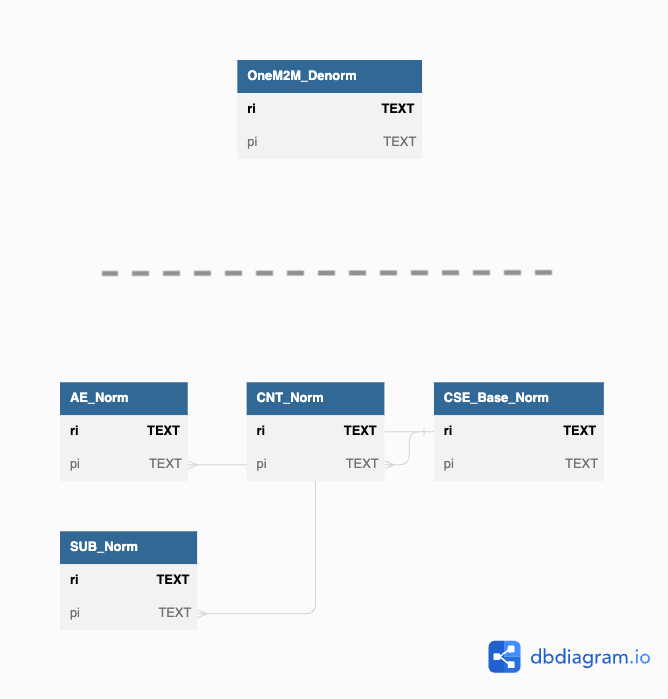
\includegraphics[width=\linewidth]{TestComparisionDBsStrategies}
	\caption{Diagram of Database Structure used for Comparison of the Normalized Strategy and Denormalized Strategy.}
	\label{fig:TestComparisionDBsStrategies}
\end{figure}

To analyze the results, let's refer to Table \ref{tab:DBComparisonResults}. For the insertion operation, the denormalized structure was slightly more time-efficient, taking an average of $6.96$ microseconds per depth layer to insert a record, while the normalized structure ranged between $6.82$ and $7.23$ microseconds per depth layer.

The selection operation showed a notable difference between the two database structures. Simple read operations on the denormalized structure consumed significantly more time (around $4500$ microseconds) than the normalized structure. However, with deep querying, the normalized structure showed an increase in operation time (up to $3300$ microseconds) due to the complexity of join operations.

In the case of the update operation, the normalized structure was slightly quicker, taking about $6.77$ to $7.32$ microseconds per depth layer compared to $6.90$ microseconds in the denormalized structure. Similar to the update operation, the delete operation was slightly faster in the normalized structure, taking between $3.67$ and $4.01$ microseconds per depth layer, while the denormalized structure took about $3.60$ microseconds.

\begin{table}[h]
\scriptsize
\centering
\caption{Average time per depth layer for CRUD operations on the databases}
\label{tab:DBComparisonResults}
\begin{tabular}{ p{1cm} p{3cm} p{3cm} }
\hline
\textbf{Operation} & \textbf{Denormalized Structure ($\mu$s)} & \textbf{Normalized Structure ($\mu$s)} \\
\hline \hline
Insert & $6.96$ & $6.82$ to $7.23$ \\
Select & $4500$ & $1.33$ to $3300$ \\
Update & $6.90$ & $6.77$ to $7.32$ \\
Delete & $3.60$ & $3.67$ to $4.01$ \\
\hline
\end{tabular}
\end{table}

From these results, we observe that the denormalized structure was more efficient in terms of insert operations, a crucial factor for applications necessitating large volumes of data insertions. However, when it comes to deep querying in a hierarchical structure, the denormalized structure outperforms due to the overhead of join operations in normalized tables. While these results are based on a relatively small example and an embedded database system, it is expected that as the database scales, these differences could become more pronounced.

\subsection{Assessing the Efficiency of Meeting Expiration Time Attribute Objectives in Database Queries on Performance}

In this part of our study, we focus on assessing the efficiency of meeting the 'expiration time' attribute objectives in database queries on performance. This test was carried out on Machine 1 shown in Table \ref{tab:machinesSpecs}, using Python version 3.9.10 and SQLite3 version 3.37.0.

The OneM2M standard can be strictly followed in certain environments, but this can sometimes lead to a degradation of system performance. A common cause for this is the inclusion of the 'expiration time' attribute and the associated logic. It's worth noting that our implementation does not delete records for which the expiration time has already passed. However, there are a couple of other possible approaches to this situation:

\begin{enumerate}
    \item \textit{On-demand Record Deletion:} All requests use the current context to search for records whose "expiration time" field has already passed and deletes them. This method adds complexity to each request, potentially impacting performance and increasing the likelihood of implementation errors.
    \item \textit{Periodic Expiration Check:} A thread is created that remains active indefinitely, checking every X time if there are fields with an exceeded "expiration time". This approach can lead to additional resource consumption and potential race conditions, making it less ideal than the first approach.
\end{enumerate}

For our test, we considered three scenarios: no implementation of the 'expiration time' attribute, implementation of the attribute without indexing, and implementation of the attribute with indexing. We chose these scenarios to demonstrate how much the presence of 'expiration time' attribute can impact the implementation, even when the attribute is indexed. We understand that there are many other ways to optimize the database statements with the presence of 'expiration time'. For instance, one could consider the use of partitioning or sharding based on expiration times \cite{Vaidya2002}, where data is logically divided into subsets based on the 'expiration time' value, thus potentially reducing the query scope and improving performance. Another could be techniques such as caching frequently accessed or recently accessed data could also be employed to improve performance \cite{Mao2012, Xing2008}. It is, however, important to note that these strategies come with their own trade-offs and complexities and should be carefully considered based on the specific requirements and constraints of the system.

A Python script was implemented to perform this test. The script created the following tables: \texttt{OneM2M\_NoET},\newline \texttt{OneM2M\_NonIndexedET}, and \texttt{OneM2M\_IndexedET}. Each table underwent 10\,000 operations of each type (Create, Read, Update, and Delete).

As shown in Figure \ref{fig:tableDiagram}, \texttt{OneM2M\_NoET} table does not implement the 'expiration time' attribute, \texttt{OneM2M\_NonIndexedET} implements it without indexing, and \texttt{OneM2M\_IndexedET} implements it with indexing. Indexing the 'expiration time' attribute can improve search times when looking for records with specific expiration times, but it also adds additional overhead when inserting or updating records, as the index needs to be updated as well.

\begin{figure}[h]
\centering
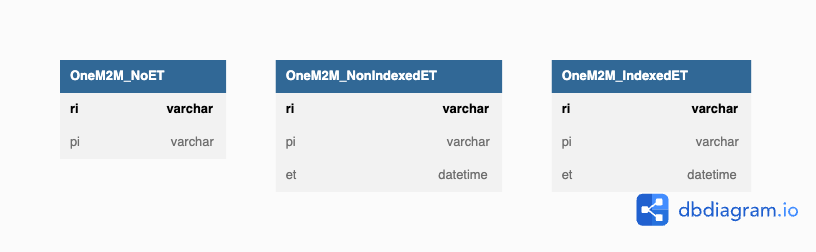
\includegraphics[width=\linewidth]{TestExpirationTime}
\caption{Efficiency of Meeting Expiration Time Attribute Test Database Tables.}
\label{fig:tableDiagram}
\end{figure}

Our results shown in Table \ref{tab:ExpirationTime} indicates that the inclusion of the 'expiration time' attribute and its indexing can degrade performance in SQLite3 database operations. Notably, the UPDATE operation was significantly slower when we considered 'expiration time', especially for the Indexed scenario. This is likely due to the overhead of maintaining the index. Similarly, for both the CREATE and DELETE operations, the presence of 'expiration time' attribute, and more so its indexing, resulted in slower operation times. These results highlight the importance of understanding the trade-offs between adhering to standards like OneM2M and the performance requirements of specific applications.

\begin{table*}[h]
\scriptsize
\centering
\caption{Results from the 'Expiration Time' test}
\label{tab:ExpirationTime}
\begin{tabular}{l p{2cm} p{2cm} p{2cm} p{2cm}}
\hline
\textbf{Scenario} & \textbf{CREATE Avg Time ($\mu$s)} & \textbf{READ Avg Time ($\mu$s)} & \textbf{UPDATE Avg Time ($\mu$s)} & \textbf{DELETE Avg Time ($\mu$s)}\\ \hline \hline
Original Codebase without Expiration Time Condition & $2.37$ & $0.976$ & $2.39$ & $0.726$\\
Non-Indexed Expiration Time Condition & $2.48$ & $1.29$ & $529\,000$ & $0.946$\\
Indexed Expiration Time Condition & $2.69$ & $1.35$ & $3\,050\,000$ & $1.09$\\ \hline
\end{tabular}
\end{table*}

\subsection{Comparative Analysis of Latency for CRUD Operations Using the Proposed Solution and OpenMTC}

In this section, we delve into a detailed test case that focuses on the comparative analysis of latency for CRUD (Create, Read, Update, and Delete) operations using the proposed solution and OpenMTC. The objective of this test case is to evaluate the performance of our solution in managing resources against the established OpenMTC standard, providing a benchmark for assessing the efficiency and effectiveness of our approach.

The CRUD operations will be performed through REST requests over the network, rather than on a local machine, as the primary goal of the oneM2M gateway is to facilitate the exchange of information across a distributed network infrastructure. This setup simulates real-world conditions where gateway systems must efficiently handle remote requests, thereby providing a more accurate representation of the solution's performance in practical applications.

To carry out this test case, the both standard implementations will be running on Machine 2, shown in Table \ref{tab:machinesSpecs}, and the requests will be done using Machine 1. The test will be conducted using a shell script that sends 500 requests affecting Content Instances, as we considered the most created resource. Because of Content Instances does not support update operations we will be doing 500 Update operations to Containers resources.

The shell script represented by Algorithm \ref{alg:time_measurement} operates as follows: It begins by initializing variables and CSV files for each CRUD operation (POST, PUT, GET, and DELETE). Then, it iterates 500 times, performing the following steps in each iteration: sending a POST, PUT, GET, and DELETE request to the respective servers and resources (CIN, and CNT), measuring the time taken for each request, and appending the time to the corresponding CSV file. After completing the 500 iterations, the script calculates the minimum, maximum, average, and standard deviation of the times for each CRUD operation from their respective CSV files. The results of these calculations provide insights into the latency of the proposed solution and OpenMTC for each CRUD operation.

\begin{algorithm}
\scriptsize
\caption{Pseudocode for Time Measurement}
\label{alg:time_measurement}
\begin{algorithmic}[1]
\State Initialize $\textit{count}$, $\textit{sum}$, $\textit{min}$, $\textit{max}$, $\textit{sq\_diff\_sum} \gets 0$
\State $\textit{min} \gets$ static large value
\For{$i \gets 1$ to $500$}
    \State Send a request to the target route
    \State Measure the time taken for the request ($\textit{time\_ms}$)
    \If{$\textit{time\_ms} < \textit{min}$}
        \State $\textit{min} \gets \textit{time\_ms}$
    \EndIf
    \If{$\textit{time\_ms} > \textit{max}$}
        \State $\textit{max} \gets \textit{time\_ms}$
    \EndIf
    \State $\textit{sum} \gets \textit{sum} + \textit{time\_ms}$
\EndFor
\State Calculate $\textit{average} \gets \frac{\textit{sum}}{500}$
\For{$i \gets 1$ to $500$}
    \State $\textit{diff} \gets \textit{time taken for request i} - \textit{average}$
    \State $\textit{sq\_diff} \gets \textit{diff} \times \textit{diff}$
    \State $\textit{sq\_diff\_sum} \gets \textit{sq\_diff\_sum} + \textit{sq\_diff}$
\EndFor
\State Calculate $\textit{standard\_deviation} \gets \sqrt{\frac{\textit{sq\_diff\_sum}}{500}}$
\end{algorithmic}
\end{algorithm}

\begin{table}
\scriptsize
\centering
\caption{Comparative Analysis of time measure for CRUD Operations in TinyOneM2M and OpenMTC.}
\label{tab:ComparativeAnalysis}
\begin{tabular}{lcccc}
\hline
& \multicolumn{2}{c}{TinyOneM2M} & \multicolumn{2}{c}{OpenMTC} \\
\cline{2-3} \cline{4-5}
Operation & Min (ms) & Max (ms) & Min (ms) & Max (ms) \\
\hline
POST & 0.123773 & 1.140625 & 0.011947 & 15.606682 \\
GET & 0.011656 & 0.115155 & 0.008696 & 1.075310 \\
PUT & 0.116248 & 0.592979 & 0.012049 & 0.136800 \\
DELETE & 0.122092 & 0.544047 & 0.008289 & 0.053867 \\
\hline
\end{tabular}
\end{table}

In a comparative analysis of latency for CRUD operations between TinyOneM2M and OpenMTC shown in Table \ref{tab:ComparativeAnalysis}, significant differences were noted. TinyOneM2M displayed a lower maximum latency for POST operations (1.140625ms) compared to OpenMTC's higher maximum (15.606682ms), suggesting more stable performance. Conversely, OpenMTC demonstrated a quicker response under optimal conditions, outperforming TinyOneM2M in terms of minimum latency for all CRUD operations, for instance, the minimum latency for GET operations was 0.008696ms for OpenMTC compared to 0.011656ms for TinyOneM2M. Further, TinyOneM2M showed less variation in response times across operations, indicating more predictable and stable performance, which could be advantageous in real-world scenarios. However, occasional latency spikes might be an issue with OpenMTC, as suggested by its high maximum latency, potentially affecting overall performance.

\subsection{Cross-Platform Evaluation: Installation and Compilation on Ubuntu, macOS, and Raspbian Operating Systems}

This section expands our cross-platform evaluation of the proposed solution to include a third operating system, Raspbian. The objective is to ensure seamless integration across diverse operating environments, underlining the solution's versatility and adaptability. This cross-platform evaluation, integral in computer science, tests the portability and interoperability of the solution across Ubuntu, macOS, and now Raspbian, catering to a broader range of users and applications.

The test case involves the installation of necessary dependencies, compilation of the source code, and execution of the proposed solution on all three operating systems, with a focus on identifying platform-specific issues. The insights gained from this evaluation will help refine the solution, ensuring its robustness and broad applicability in the context of the oneM2M standard.

The source code was imported to all machines, that use one of each operating system addressed in this section, shown as Table \ref{tab:machinesSpecs}, and the solution was successfully installed and compiled on all machines, leveraging the pre-installed GCC compiler. The Makefile facilitated the compilation, resulting in the creation of the executable without complications. An interesting observation is that the resultant executable file across all the operating systems maintained a consistent size of 1.4Mb, which indicates a uniform and efficient code compilation and linking process. Dependencies of the compiled executable were examined using the \texttt{ldd} and \texttt{otool} commands, revealing an exclusive reliance on system libraries.

The solution's dependence on system libraries alone, such as \texttt{libdl.so.2}, \texttt{libpthread.so.0}, and \texttt{libc.so.6} for Ubuntu and Raspian, and only \texttt{libSystem.B.dylib} for macOS simplifies the installation process and enhances portability and maintainability across platforms. It also benefits from the stability and performance optimizations provided by the operating system's native libraries.

This successful installation, compilation, and dependency identification demonstrates the adaptability of our solution to different operating environments. This adaptability is crucial in ensuring the software's portability and interoperability across different platforms, broadening its potential user base.

Our solution exhibits impressive cross-platform compatibility, having been successfully installed and compiled on Ubuntu, macOS, and Raspbian. The primary reliance on system libraries boosts its portability and maintainability, simplifying the process across various platforms. This reinforces the potential for broad adoption of the solution and the importance of designing versatile software across diverse platforms.

However, while we remain confident about the straightforward installation of the solution on most Linux-based operating systems, additional steps may be required to support Windows, such as an abstraction layer for the pthread library. This highlights the continual need for refinement and adaptation to ensure comprehensive cross-platform compatibility.

\subsection{Minimal Hardware Compatibility Testing: Raspberry Pi 0 W Case Study}

In this section, we present a case study using the Machine 3 microcontroller, as shown in Table \ref{tab:machinesSpecs}. Our objective is to test the compatibility of our proposed solution with resource-constrained environments. This test will be conducted using minimal hardware, an essential consideration in computer science, as many real-world applications require efficient and lightweight solutions capable of running on devices with limited processing power, memory, and energy resources.

The hardware selected for this test is a Raspberry Pi 0 W, a cost-effective and popular microcontroller with integrated Wi-Fi and Bluetooth capabilities. For storage, we used a Kingston 64GB SD Card with a read speed of 100MB/s, a suitable choice for our test scenario.

Our experiment was designed to create SQLite3 CIN resources in quantities of 10\,000, 50\,000, and 100\,000, storing them in the database located on the SD card. We measured the size of the database on the disk and the RAM usage when all resources were loaded by our server application. The shell script we used executed SQLite3 commands to create the desired number of resources and measured the database size, while the top command measured RAM usage, targeting our server application process. The results of these measurements are tabulated in Table \ref{tab:ResourceUtilization}.

\begin{table}[h]
\scriptsize
\centering
\caption{Resource Utilization for Different Numbers of Content Instance Resources on Raspberry Pi 0 W.}
\label{tab:ResourceUtilization}
\begin{tabular}{ p{1.5cm} p{2.5cm} p{2.5cm} }
\hline
\textbf{Instances} & \textbf{Database Size (KB)} & \textbf{RAM Usage (KB)} \\
\hline \hline
10\,000 & 9\,136 & 5\,608 \\
50\,000 & 46\,336 & 9\,696 \\
100\,000 & 92\,984 & 14\,772 \\
\hline
\end{tabular}
\end{table}

The outcomes of this test case provide significant insights into real-world scenarios, especially those where resources are limited. The efficiency of a solution in such circumstances is determined by its ability to perform effectively under these constraints. These tests can help us understand the suitability of our solution in such situations, and also provide a basis for further optimization.

It's important to note that the recorded RAM usage and disk space are the results of operating in a controlled environment. Actual values can vary depending on a number of other factors, including the specifics of the implementation, the operating conditions, and the additional overhead imposed by other running processes and OS services. Nevertheless, this experiment serves as a valuable indicator of the resource efficiency of our solution.

\section{Lessons Learned}
\label{sec:lessonsLearned}

In the pursuit of technological innovation, it is not uncommon to traverse uncharted territory and learn through trial and error. This document, reflecting on our journey with the implementation of the TinyOneM2M project, endeavors to impart the lessons we have gleaned, offering readers a distilled version of our experiences and the wisdom we have accrued. This section will broadly focus on key areas such as our choice of database technology, database structure, the use of libraries, and the implementation of the OneM2M standard, each accompanied by the lessons learned and the strategies we adopted for overcoming challenges.

During the development stage, we opted for a single file database over a server-based database, believing it would offer superior performance. However, as we progressed, we discovered that this assumption might not hold. The performance gains we expected did not materialize, prompting us to reevaluate our choice of database technology and explore alternative options, such as a MySQL database because of concurrency, and high write rate, on the other hand, would increase the size of the executable because of the size package size, and the database size occupied.

Following established database best practices, we initially pursued a normalization approach for our database structure which involved creating two tables: "mtc" and "multivalue." The introduction of the multivalue table played a vital role in our database structure since it facilitated the mapping of intricate dependency relationships between each \gls{m2m} resource. This approach proved particularly valuable in handling the dynamic and complex nature of \gls{json} relationships, enabling us to effectively represent the infinite-like associations that can exist within \gls{json} values. While this approach adhered to standard guidelines, it downgrades performance due to the time-consuming processing required to map a \gls{json} structure in C into corresponding database entries significantly impacting the overall performance of our system. Consequently, we recognized that denormalization would be a more suitable strategy for our project, allowing for improved performance and streamlined data retrieval. Therefore, this ultimately became the final approach we chose to implement our database.

Another of the lessons we learned relates to using static C libraries. While these libraries offer certain advantages, such as ease of distribution and reduced dependency management, they pose challenges when keeping up-to-date with new versions. On the positive side, static libraries provide a stable and predictable development environment. However, the downside is that they do not benefit from bug fixes, security patches, or new features introduced in subsequent releases. This trade-off necessitates careful consideration and evaluation of the specific project requirements when choosing between static and dynamic libraries.

Implementing the OneM2M standard involved incorporating various attributes, including expiration time (et), maximum byte size (mbs), and maximum number of instances (mni), among others. While these attributes align with the standard, their inclusion increases implementation complexity and hinders performance. Moreover, in practical scenarios, these fields often have little relevance or are not frequently utilized. Therefore, the attributes to implement must be extensively evaluated to strike a balance between adherence and practicality.

\section{Conclusion and Future Work}
\label{conclusion}

In this section, we will discuss the conclusions drawn from our C implementation of OneM2M and outline the potential areas for future work and improvement.

To overcome the limitations associated with high-level language-based implementations, we present a novel approach by leveraging a low-level programming language for the implementation of the OneM2M standard. Our methodology aims to address the challenges posed by the evolving \gls{iot} landscape, with a particular focus on \gls{mtc} gateways. By emphasizing crucial aspects like protocol interoperability, scalability, and latency, our implementation offers improved performance, reduced memory overhead, and enhanced control over hardware resources. Through comprehensive testing, we thoroughly assessed the efficacy, usability, scalability, and reliability of the TinyOneM2M solution in various scenarios. Our findings validate its suitability as a robust and efficient solution for meeting the demands of the \gls{iot} ecosystem.

The Home Gateway Scenario, the Single Devices Scenario (peer-to-peer), and the Cloud Scenario are the three main scenarios supported by TinyOneM2M's system architecture. TinyOneM2M functions as a central gateway within a home network in the Home Gateway Scenario, facilitating communication between various devices. The scenario for single devices is a decentralized method in which each device has its own instance of TinyOneM2M, allowing for direct connection between devices without the need for a centralized communication hub. In the cloud scenario, TinyOneM2M is hosted by a cloud provider, enabling large-scale dispersed \gls{iot} applications by enabling device connectivity and internet communication. 

Our TinyOneM2M solution implementation follows to version 5.1 of the OneM2M standard and concentrates on important resources including CSE\_Base, AE, CNT, CIN, and SUB. The C programming language, which offers portability and efficiency for \gls{iot} applications, was used to construct the solution. However, it requires careful memory management and lacks built-in object-oriented capabilities. Also, the fact of in media our implementation covers 57\% of the standard is very promissory. As the embedded single file database, we used SQLite3, which offered dependable data persistence and effective retrieval techniques. Performance was enhanced by the denormalized, single-table design, although for particular circumstances, other database options like MySQL or PostgreSQL might be taken into consideration.

Our tests yielded several noteworthy outcomes. The implementation of the TinyOneM2M solution proved to be highly reliable, effectively addressing the interoperability and communication demands within an \gls{iot} ecosystem. Interacted with various platforms, protocols, and devices, facilitating efficient resource management and few effort data transmission. 

The solution showcased impressive scalability, exhibiting consistent performance even with an increasing number of connected devices and growing data traffic. This scalability is vital for accommodating the expanding \gls{iot} landscape, ensuring the system's ability to handle large-scale deployments and accommodate future growth. This solution has potential for enterprises looking for effective management of their \gls{iot} ecosystems as \gls{iot} continues to develop and grow.

Overall, TinyOneM2M's architecture offers a reliable and effective mechanism for putting the OneM2M standard into \gls{iot} contexts. It allows for seamless communication and data management in \gls{iot} applications by providing flexibility, scalability, and ease of integration into diverse scenarios. The TinyOneM2M solution we implemented shows a strong foundation and significant advancement towards the OneM2M standard. Platform independence, performance, and resource coverage can all be further improved and enhanced.

Future endeavours encompass various areas where our implementation of OneM2M can be further refined and enhanced. Currently, there is no validation to ensure that the content of the request body is a \gls{json}, therefore potentially leading to erroneous or inconsistent data in the requests. To fix this issue it's mandatory to ensure that the request contains a \gls{json} object as the request body type. 

Secondly, the current implementation doesn't fully guarantee the integrity and accuracy of the received data since only a few attributes of the standard's resources are being validated (e.g. expiration time, URI and RN). Therefore, future work consists of performing attribute validation for all the resource's attributes passed in the \gls{json} body of the requests.

During the implementation process, ensuring compatibility with Windows systems posed a persistent challenge, primarily due to the absence of the pthread library, which is specific to Unix systems. As a result, alternative libraries, such as pthreads-w32, would need to be employed when working with Windows systems. Consequently, a crucial future task is to develop an abstraction layer that enables cross-platform compatibility. By abstracting the thread implementation, we can enhance its portability and accessibility and ensure the execution of our implementation on diverse operating systems.

Moreover, given the extensive scope of the OneM2M standard, numerous resources have not yet been developed. Currently, only a partial implementation of the CSE\_Base, \gls{ae}, \gls{cnt}, \gls{cin}, and \gls{sub} resources has been accomplished. Therefore, a vital area for future work is to complete the implementation of the standard, ensuring that all the resources outlined in the OneM2M standard are fully developed. This undertaking is crucial to provide a more comprehensive and feature-rich implementation of OneM2M, enabling a broader range of functionalities and accommodating a wider array of use cases.

Lastly, TinyOneM2M is currently at the margin of having concurrency problems in a multi-threaded environment. Therefore, it would be advantageous to improve the transactional behaviour with write-ahead logging (WAL) or other techniques to enhance concurrency. Additionally, our system could also be optimized at a database attribute level by performing deep analysis and study of the SQLite3 database operations and available operators such as PRAGMA.

Overall, these future enhancements will further solidify our implementation and ensure its effectiveness in the \gls{iot} ecosystem.


%% Loading bibliography style file
%\bibliographystyle{model1-num-names}
%\bibliographystyle{cas-model2-names}
\bibliographystyle{unsrt} % Estilo de Bibliografia
% Loading bibliography database
\bibliography{cas-refs}


%\vskip3pt

\end{document}
